\newcommand{\pd}[2]{\displaystyle\frac{\displaystyle\partial #1}{\displaystyle\partial #2}}
\newcommand{\vol}[1]{\langle #1 \rangle}
\newcommand{\sigy}{\sigma_{\rm y}}
\newcommand{\epse}{\varepsilon^{\rm e}}
\newcommand{\epsp}{\varepsilon^{\rm p}}

\newcommand{\epst}{\varepsilon}
\newcommand{\sig}{\sigma}
\newcommand{\Fp}{f^{\rm p}}
\newcommand{\Fd}{f^{\rm d}}
\newcommand{\norm}[1]{| #1 |}

\section{Motivation}

\frame{\frametitle{Fatigue damage}

\uncover<1->{
		\twocol{	\begin{itemize}
				\item Cyclic loading
			\end{itemize}
			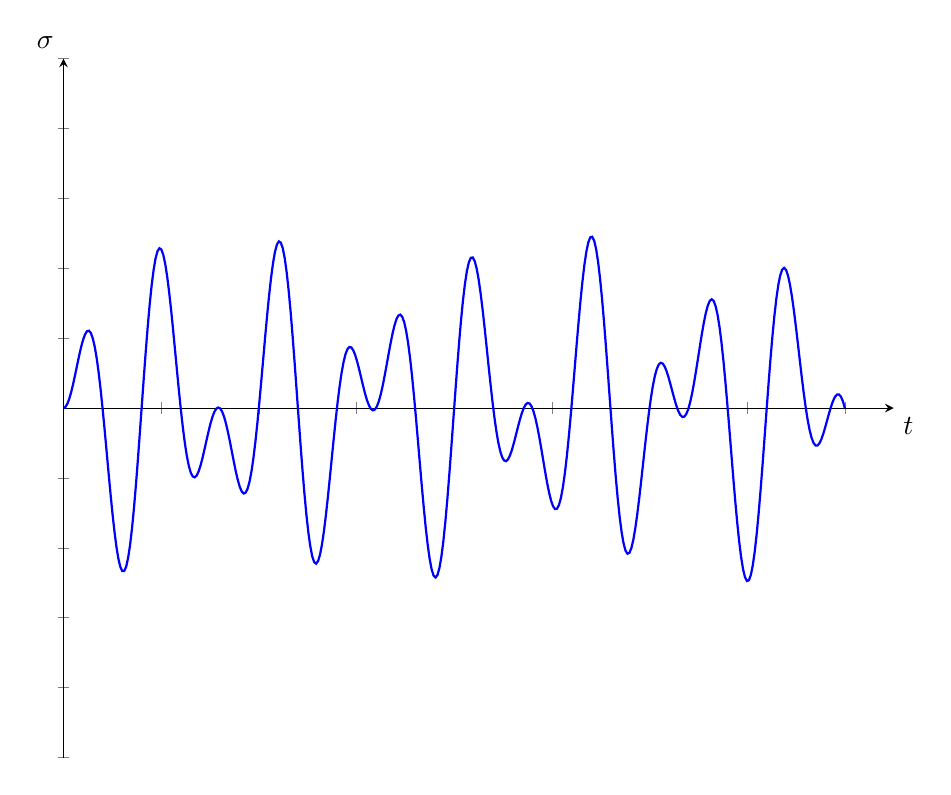
\begin{tikzpicture}[scale=1]
			\begin{axis}[axis x line=center, axis y line=center,
			xticklabels={},yticklabels={},xlabel style={below right},
			ylabel style={above left},ymin=-1,ymax=1,xmin=0,xmax=8.5,
			width=\textwidth,xlabel=$t$,ylabel=$\sigma$]
			\addplot [color=blue,thick,mark=none,domain=0:8,samples=400]{sin(2*\x r)*0.5*sin(pi / 2 * 5 * \x r)} ;
			\end{axis}
			\end{tikzpicture}
		}{
			\centering
			\uncover<2->{\hfil
				\begin{itemize}
					\item Damage
				\end{itemize}
				
					\only<2>{\includegraphics[width=0.9\textwidth]{./img/Windturbine.jpg}\\[-0.3cm]}

					\only<3->{\includegraphics[width=0.9\textwidth]{./img/bridge.jpg}\\[-0.3cm]}
						
									{\tiny Image by alegri / 4freephotos.com}
					\uncover<4>{	\begin{tikzpicture}[x=1cm,y=1cm,overlay]
						\node [draw,fill,circle,radius=1pt,inner sep=0.5pt] at (-0.7,1.5) {};
						\draw (-2,-0.3) -- (-0.7,1.5);
						\draw (-0.5,-0.3) -- (-0.7,1.5);
						\draw (-2,-1.8) -- (-0.7,1.5);
						\draw (-0.5,-1.8) -- (-0.7,1.5);
						\draw [thick,fill=white] (-2,-1.8) rectangle ++(1.5,1.5);
						\node [draw,circle,radius=1pt,inner sep=1.5pt] at(-1.5,-1.5) {};
						\draw (-1,-1.1) ellipse (0.5mm and 3mm);
						\node [draw,circle,radius=1pt,inner sep=1.5pt] at(-1.5,-0.6) {};
						\draw [->,thin] (-.5,-1.1) -- ++(0.6,0) node [below right,pos=0.5] {$\sigma$};
						\draw [->,thin] (-2,-1.1) -- ++(-0.6,0) node [below left,pos=0.5] {$\sigma$};
						\end{tikzpicture}}
				}
				
				}
			}
			{
			
			}
	}



\frame{\frametitle{Fatigue damage}
	
		\twocol{	\begin{itemize}
				\item Cyclic loading
			\end{itemize}
			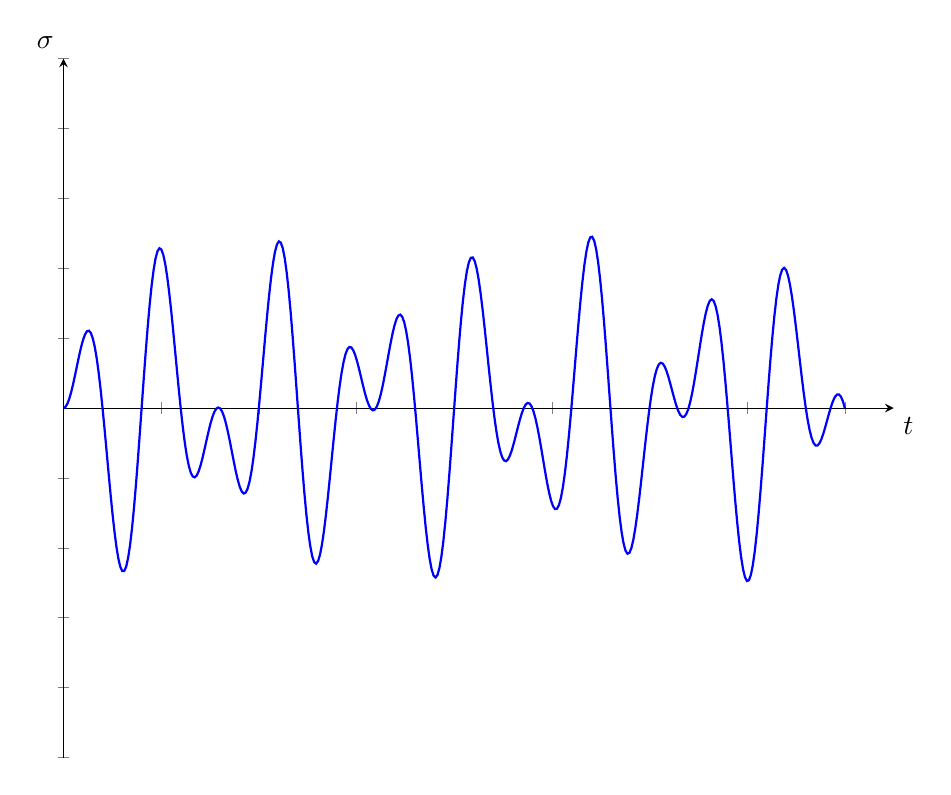
\begin{tikzpicture}[scale=1]
			\begin{axis}[axis x line=center, axis y line=center,
			xticklabels={},yticklabels={},xlabel style={below right},
			ylabel style={above left},ymin=-1,ymax=1,xmin=0,xmax=8.5,
			width=\textwidth,xlabel=$t$,ylabel=$\sigma$]
			\addplot [color=blue,thick,mark=none,domain=0:8,samples=400]{sin(2*\x r)*0.5*sin(pi / 2 * 5 * \x r)} ;
			\end{axis}
			\end{tikzpicture}
		}{
			\centering
			\uncover<1->{\hfil
				\uncover<1->{	\begin{itemize}
						\uncover<1->{\item Virtual experiments\\[0.5cm]}
						\uncover<2->{\item Continuum damage model\\[0.5cm]}
						\uncover<3->{\item Millions of cycles\\[0.5cm]}
						\uncover<4->{\item Computationally expensive\\[0.5cm]}
					\end{itemize}}	
				}
			}
			{
				\uncover<5>{
					\begin{block}{ \centering Model order reduction (MOR) techniques}
					\end{block}
					
				}
			}
		}

	
\frame{
	\frametitle{Model order reduction (MOR)}
\begin{itemize}
	\item Proper orthogonal decomposition (POD) \\[-0.2cm]
		{\hspace*{0.3cm} \tiny [Antoulas 2005; Quarteroni, Manzoni, Negri 2016 ]}\\
		\pause
\uncover<2->{	\item Proper generalised decomposition (PGD) \\[-0.2cm] {\hspace*{0.3cm} \tiny [Ladeveze 1985,1999; Chinesta, Ladev{\`e}ze 2014]}\\
%	[Ladeveze 1985,1999; Chinesta, Ladev{\`e}ze 2014]}\\
	$\hfil \epsp(x,t) \approx \sum_{i=1}^{n} \bar{\varepsilon}^{\rm p}(x) \ \lambda(t)$
	
	\uncover<3->{\begin{itemize}
		\item Intrusive method
		\item Integrals over the generalised coordinates\\[1cm]
	\end{itemize}}}
	\uncover<4>{	\begin{block}{\centering Need for a convenient framework to utilise PGD}
		\end{block}}
\end{itemize}
}
	
\section{LATIN framework}

\frame{\frametitle{Large time increment (LATIN) method }
		\begin{itemize}
			\item{At each iteration}\\
%		\scriptsize
		{\footnotesize $\bullet$ An approximation on the \textbf{whole time-space domain} is obtained.} \\	
		{\footnotesize $\bullet$ The balance equation is solved as a \textbf{linear} problem.} 
	\end{itemize}
		
			\only<2>{
				\begin{center} 
				\animategraphics[loop,width=0.5\linewidth,height=2in,autoplay]{1}{./img/lating-}{0}{14}
			\end{center}
				}
%		\mediabutton[jsaction={anim.myAnim.playFwd();}]{\fbox{\strut Play}}
%		\mediabutton[jsaction={anim.myAnim.pause();}]{\fbox{\strut Pause}}
	%		 \includegraphics[width=0.4\linewidth]{./img/lating-0.png}
\vfill
}



\frame{\frametitle<1-3>{The LATIN framework}
	\frametitle<4->{The LATIN iterative scheme}
%	\framesubtitle<1,4>{ \quad \color{white} 00000}
%	\only<2>{\framesubtitle{iteration $i+1/2$}}
%	\only<3>{\framesubtitle{iteration $i+1$}}
%	%	\begin{center}
%	%\vspace*{1cm}
%	\hspace*{-0.5cm}
%	\uncover<1->{\begin{minipage}[t]{0.6\linewidth}		


\twocol{

	\begin{flushleft}
	\only<1>{\vspace*{1cm}
		\begin{itemize}
			\item {Assumptions}\\[0.2cm]
			\begin{itemize}
				\item Free energy function $\psi$\\
				\Sbf{State equations}
				\item Dissipation potential $\phi$
				\Sbf{Evolution equations}\\
				\item Here: no dynamic effects \\[0.4cm]
			\end{itemize}
		\end{itemize}
		
		\begin{itemize}
			\item Linear initialisation\\[0.2cm]
			\qquad $		\epst = \epse$
		\end{itemize}	
	}
	\only<2>{
		\begin{itemize}
			\item {\color{red} Non-linear step}\\[0.3cm]
			\item The evolution equations\\[0.3cm]
			\hfil e.g. ${\dot {X}} =- \pd{\phi}{{Y}} $\\[0.3cm]
			\item {\color{red} Local in space} (cheap)\\[0.3cm]
%			\item Suitable for parallelisation
		\end{itemize}	
	}
	
	\only<3>{
		\begin{itemize}
			\item  {\color{blue} Linear step}\\[0.3cm]
			\item {The equilibrium equation }\\[0.3cm]
			\hfil ${\rm div}(\boldsymbol{\sigma}) = \boldsymbol{0}$ \\[0.3cm]
			\item  {\color{blue} Global in space}\\[0.3cm]
			\item Convenient to apply PGD			

			%			$\int_{t} \int_{\Omega} \sigma : \varepsilon \ {\rm d}\Omega \ {\rm d}t = ....$
			%			\item Integrate iteratively over time and space domains\\
			%			$  \Delta \epsp(x,t) \approx \sum_{i=1}^{n} \bar{\varepsilon}^{\rm p}(x) \ \lambda(t) $
			%			\item Update time functions
			%			\item If needed add only one pair per iteration
		\end{itemize}	
	}

\end{flushleft}
}{

	\newcommand{\cA}{{\cal A}}
\begin{flushleft}
	\begin{tikzpicture}[x=1cm,y=1cm,overlay]
	\node at(2,-1) {\begin{tikzpicture}[xscale=0.9,yscale=0.9]
		%\draw [help lines] (0,0) grid (7,7);
		\uncover<1->{\draw [name path=evolution, rotate=-15,ultra thick,postaction={decorate,decoration={text along path,raise=1ex,text align=center,text={|\small  | Evolution equations}}}] (1,0) arc [radius=10,start angle=160, end angle=120] node[above] {$\Gamma$};}
		\uncover<2->{\path [rotate=-15,ultra thick,postaction={decorate,decoration={text along path,raise=1ex,text align=center,text={}}}] (1,0) arc [radius=10,start angle=160, end angle=120] (1,0) arc [radius=10,start angle=160, end angle=120]
			node[pos=0.75,circle,radius=1pt,fill=blue,inner sep=1.5pt] (s1)  {} ;}
		\uncover<1->{\begingroup
			\footnotesize 
			\draw [name path=KA_SA, ultra thick] (0.5,0.5) -- (7,1.2) node[pos=0.55,sloped,below,align=left]{\baselineskip=8pt Kinematic admissibility \\ Static admissibility \\ State equations} node[above] {$\cA$};
			\endgroup}
		\uncover<1->{
			\path (0.5,0.5) -- (7,1.2) 
			node[pos=0.9,circle,radius=1pt,fill=red,inner sep=1.5pt] (s0) {}	;}
		% node[label={[label distance=-0.25cm]30:$s_0$}] at (s0) {}
		\uncover<3->{
			\path (0.5,0.5) -- (7,1.2) 
			node[pos=0.685,circle,radius=1pt,fill=red,inner sep=1.5pt] (s2) {};	  ;}
		\uncover<2->{\draw [>=latex,->,thick,red] (s0) -- (s1) node[pos=0.5,sloped,above,red]{} node [pos=0.4,sloped,below] {};}
		\uncover<3->{\draw [>=latex,->,thick,blue] (s1) -- (s2) node[pos=0.5,sloped,above,blue]{} node [pos=0.6,sloped,below] {};}

		
		\end{tikzpicture}};
\end{tikzpicture}
\end{flushleft}

}
{}
}





\section{MOR for damage}

\frame{\frametitle{LATIN with isotropic damage}
	\twocol{
		\vspace*{0.8cm}
		\begin{itemize}
			\item {State equation} \\[0.1cm]	
				{e.g. \hfil $ \boldsymbol{\sig}= E \ {\color{red} (1-D)} \ \boldsymbol{\epse}$} \\[0.1cm]	
			\uncover<2->{\item Nonlinear $\cal A$ \\[0.3cm]}

		\uncover<3->{\Sbf{Workaround}\\[0.3cm]

		\item Solve
		{\hfil $ \boldsymbol{\sig}= E \ {\color{red} (1-D)} \ \boldsymbol{\epse}$} \\[0.1cm]
		\hfil in the {\color{red} local step}\\[0.1cm]}
		
		\uncover<4>{
		\item Linear $\cal A$\\[0.1cm]
		
		\item Use {\color{Sbluea}PGD} for the global step}

		\end{itemize}

 }{
\newcommand{\cA}{{\cal A}}

\hspace*{-1cm}
	\begin{tikzpicture}
	\node at(2,-2.8) {\begin{tikzpicture}[x=1cm,y=1cm,xscale=0.9,yscale=0.9]
%		%\draw [help lines] (0,0) grid (7,7);
		\uncover<1->{\draw [name path=evolution, rotate=-15,ultra thick,postaction={decorate,decoration={text along path,raise=1ex,text align=center,text={|\small  | $ \ \ \ \ \ \ \ \ $ Evolution equations}}}] (1,0) arc [radius=10,start angle=160, end angle=120] node[above] {$\Gamma$};}
%		\uncover<4>{\draw [name path=evolution, rotate=-15,ultra thick,postaction={decorate,decoration={text along path,raise=1ex,text align=center,text={|\small| Evolution equations }}}] (1,0) arc [radius=10,start angle=160, end angle=120] node[above] {$\Gamma$};}		
%		\uncover<4>{\draw [name path=evolution, rotate=-15,ultra thick,postaction={decorate,decoration={text along path,raise=1ex,text align=center,text={|\small  | $ \ \ \ \ \ \ \ \ $ Evolution equations, $\sigma$ state eq.}}}] (1,0) arc [radius=10,start angle=160, end angle=120] node[above] {$\Gamma$};}
		\uncover<2-3>{\draw [name path=evolution, rotate=-50,ultra thick,postaction={decorate,decoration={text along path,raise=1ex,text align=center,text={|\small| $ \ \ \ \ \ \ \ \ \ \ $ Admissibility, State eq.}}}] (0.2,0.8) arc [radius=10,start angle=160, end angle=125] node[above] {$\cA$};}		
		\uncover<4>{
			\draw [name path=KA_SA, ultra thick] (0.8,0.4) -- (6.8,0.7) node[pos=0.55,sloped,below,align=left]{Admissibility, Hard. state eq.} node[above] {$\cA$};
			}
%%		Kinematic admissibility \\ Static admissibility \\ State equations
		\end{tikzpicture}};
		\end{tikzpicture}
}{}}

\frame{\frametitle{PGD}
	$\hfil {{\varepsilon}}^{\rm p}(x,t) \approx \sum_{i=1}^{n} {\lambda}(t) \ \bar{\varepsilon}^{\rm p}(x) $	\\

\begin{algorithm}[H]
%	\KwData{this text}
%	\KwResult{$\lambda(t), \bar{\varepsilon}^{\rm p}(x)$ }
	Initialise ${\lambda}(t)$\\
	\While{\texttt{err}$>$\texttt{tol}}{
		compute the space function $\bar{\varepsilon}^{\rm p}(x) \longleftrightarrow$  $\int_t \bullet \ dt$\\
		compute the time function $\lambda(t) \longleftrightarrow$  $\int_\Omega \bullet \ d\Omega$
}
\hfil {\textbf{ALgorithm: }PGD enrichment step}
\end{algorithm}
\uncover<2>{\begin{itemize}
		\item Auto. generation of the best pairs by a greedy algorithm
		\item No a priori assumption on the reduced order basis 
	\end{itemize}
	}
%	\begin{algorithm}
%		Initialise $\dot{\lambda}(t)$\;
%	\end{algorithm}
	
}
\section{Numerical example}

\frame{\frametitle{Numerical example}
	
	\begin{itemize}
		\item  Chaboche Marquis constitutive model {  \tiny [Chaboche 1993; Cognard 1993]}\\[-0.1cm]
			{\scriptsize (Cr-Mo steel at $580^\circ {\rm C}$,  Unilateral damage, isotropic hardening)}\\[-1cm]
	\end{itemize}
%\pgfdeclarehorizontalshading{rainbow}{100bp}{%
%	rgb(0bp)=(1,0,0);
%	rgb(26bp)=(1,0,0);
%%	rgb(33bp)=(1,.5,0);
%	rgb(40bp)=(1,1,0);
%%	rgb(47bp)=(0,1,0);
%	rgb(54bp)=(0,1,1);
%	rgb(61bp)=(0,0,1);
%	rgb(68bp)=(1,0,1);
%%	rgb(75bp)=(.5,0,.5);
%	rgb(100bp)=(.5,0,.5)}
\begin{center}
	\begin{tikzpicture}[x=1cm,y=1cm,scale=0.7]
	
{ \small
	\node at (4,-2) [align=left]	{
	\only<1>{$\ \psi = \frac{1}{2} \ E \ (\epse)^2 + \underset{\text{hardening}}{\underbrace{ \frac{1}{2} \ C \ (\alpha)^2}} $\\[0.2cm]}
	\only<2->{$\psi = \frac{1}{2} \ E \ (\epse)^2 \ {\color{red} (1-D)} + \underset{\text{hardening}}{\underbrace{ \frac{1}{2} \ C \ (\alpha)^2}}$\\[0.2cm] \hspace*{0.0cm}}
	$\phi=\phi^{\rm p} \uncover<3->{+ \color{red}  \phi^{\rm d}}$\\[0.2cm]
	\begin{tabular}{ll}
	$ \phi^{\rm p}= \frac{k}{n+1} \vol{f^{\rm p}}_+^{n+1}$ & $f^{\rm p} = \norm{\sigma - \beta} + \frac{a}{C} \ \beta^2 - \sigy$ \\[0.2cm]
	\uncover<4->{$ \phi^{\rm d} = \frac{\kd}{\nd+1} \vol{\Fd}_+^{\nd+1}$ &  $ \Fd=Y-Y_0$}
	\end{tabular}

	};
}
	\fill [ultra thick] (0,-0.05+1.75) rectangle (4,0.05+1.75) node [above,pos=0.5] {};
	\fill [ultra thick] (0,-0.05+1.25) rectangle (4,0.05+1.25) node [above,pos=0.5] {};
	\fill [thick] (4,-0.05+1.25) rectangle (4.05,0.05+1.75) node [above,pos=0.5] {};
	
	\draw [->,thin] (4,0+1.5) -- (4.5,0+1.5) node [below right,pos=0.5] {$\bar{u}$};
	\draw [ultra thick] (0,-0.5+1.5) -- (0,0.5+1.5);
	\path [pattern=north west lines] (-0.25,-0.5+1.5) rectangle (0,0.5+1.5);
	\begin{axis}[at={(0.6\textwidth,-2)},axis x line=center, axis y line=center,
	xticklabels={},yticklabels={},xlabel style={below right},
	ylabel style={above left},ymin=-1,ymax=1,xmin=0,xmax=8.5,
	width=0.5\textwidth,xlabel=$t$,ylabel=$\bar{u}$]
	\addplot [color=blue,thick,mark=none,domain=0:8,samples=400]{0.5*sin(pi / 2 * 5 * \x r)} ;
	\end{axis}
	\end{tikzpicture}\\
%	{ \tiny Uniaxial visco-plastic bar with cyclic loading without considering dynamic effects}\\[0.5cm]
\end{center}}

\frame{\frametitle{The convergence behaviour}
	\vfill
	
	\twocol{\hspace*{-0.6cm} \input{img/damage_error.tex}\\
%		\hspace*{1cm} \fontsize{10}{12}\selectfont Error decrease
	}{\hspace*{-1.cm}
		\includegraphics[width=1.15\textwidth,clip]{img/damage_d.png}\\
		\centering {\scriptsize Damage evolution at convergence}}{}
}

\frame{\frametitle{The plastic strain evolution using PGD}
	\input{img/damage_pairs}
	\hspace*{0.2cm}
	\begin{tikzpicture}[overlay]
	\tiny
		\node at (0.7,3.9) {$\times$};
		\node at (1.6,3.9) {$+$};
		\node at (2.6,3.9) [align=center] {time function \\ $\times$ \\ space function};
		\node at (3.5,3.9) {$+$};
		\node at (4.4,3.9) {$\times$};
		\node at (5.3,3.9) {$=$};
	\end{tikzpicture}
	$\hfil {\dot{\varepsilon}}^{\rm p}(x,t) \approx \sum_{i=1}^{3} \dot{\lambda}(t) \ \bar{\varepsilon}^{\rm p}(x) $
} 

\frame{ \frametitle{Conclusion and current research}
	
	\vspace*{-1cm}
	
		\fboxsep=0pt
		
		\begin{tikzpicture}[x=1mm,y=1mm,remember picture,overlay]
		\node at (28,4) {{%
				\begin{minipage}{0.7\textwidth}
					\begin{itemize}
					\item A LATIN-based model reduction approach for
					the simulation of ductile damage { \tiny [M. Bhattacharyya et al 2017, {\textit{submitted}}]		}
					\item {Two-time scale fatigue damage framework {\tiny (\textit{in progress})}}\\%[0.4cm]	
					\end{itemize}
				\end{minipage}}};
		\node at (86,4) {{%
				\begin{minipage}{0.4\textwidth}
				\includegraphics[width=0.8\textwidth]{./img/mainak.png}\\[-0.5cm]
				\hspace*{0.5cm}\includegraphics[width=0.7\textwidth]{./img/timescale.png}	
				
				\end{minipage}}};	
		\node at (57,-35) {{%
				\begin{minipage}{1.05\textwidth}
					\uncover<2->{
						\vspace*{-1cm}
							\begin{block}{\centering Current research}
						\end{block}\vspace*{-0.5cm}
						{\begin{itemize}
							\item {Extend the two-time scale to consider}\\
							\qquad Different amplitudes, frequencies and random loadings\\
							\end{itemize}}}
					
					\uncover<3>{	\begin{block}{\centering Thank you for your attention!}
						\end{block}}
				\end{minipage}}};	
		\end{tikzpicture}
		
}

\frame{
	\begin{itemize}
		\item Time comparison\\
			 D. N\'{e}ron et al, Time-space PGD for the rapid solution of 3D nonlinear
			parametrized problems in the many-query context, \textit{IJNME}, 2015.
	\end{itemize}
	}
	



\frame{
	\begin{itemize}
		\item  PGD for solving PDE\\
		A. Nouy. A priori model reduction through proper generalized decomposition for solving time-dependent partial differential equations. Computer Methods In Applied Mechanics and Engineering, 199(23- 24):1603–1626, 2010.\\
		Antonio Falco\\
	\end{itemize}
}
	
%\frame{\frametitle{}
%	
%	}
	
\input{MOR}
%\frame{
%	\begin{itemize}
%		
%		\item PGD convergence\\
%		generalisation of the POD of a given function, is independent of the LATIN-PGD. In the book, you have this proof for a given continuous function, 
%		[Ladevèze 99] 
%		
%	\end{itemize}
%}